% ==============================================================================
% Modelo para Especificação de Projeto de Software
% Prof. Vítor E. Silva Souza - NEMO/UFES :: DI/UFES :: PPGI/UFES
%
% Baseado em abtex2-modelo-trabalho-academico.tex, v-1.9.2 laurocesar
% Copyright 2012-2014 by abnTeX2 group at http://abntex2.googlecode.com/ 
%
% This work may be distributed and/or modified under the conditions of the LaTeX 
% Project Public License, either version 1.3 of this license or (at your option) 
% any later version. The latest version of this license is in
% http://www.latex-project.org/lppl.txt.
%
% IMPORTANTE:
% Instruções encontram-se espalhadas pelo documento. Para facilitar sua leitura,
% tais instruções são precedidas por (*) -- utilize a função localizar do seu
% editor para passar por todas elas.
% ==============================================================================

% Usa o estilo abntex2, configurando detalhes de formatação e hifenização.
\documentclass[
	12pt,				
	oneside,		
	a4paper,			
	english,			% Idioma adicional para hifenização.
	french,				% Idioma adicional para hifenização.
	spanish,			% Idioma adicional para hifenização.
	brazil				% O último idioma é o principal do documento.
	]{abntex2}


%%% Importação de pacotes. %%%

% Conserta o erro "No room for a new \count". 
% O comando \reserveinserts deve ser comentado ou não, dependendo da versão do LaTeX.
\usepackage{etex}
%\reserveinserts{28}

% Usa a fonte Latin Modern.
\usepackage{lmodern}

% Seleção de códigos de fonte.
\usepackage[T1]{fontenc}

% Codificação do documento em Unicode.
\usepackage[utf8]{inputenc}

% Usado pela ficha catalográfica.
\usepackage{lastpage}

% Indenta o primeiro parágrafo de cada seção.
\usepackage{indentfirst}

% Controle das cores.
\usepackage[usenames,dvipsnames]{xcolor}

% Inclusão de gráficos.
\usepackage{graphicx}

% Melhor controle de leiaute de tabelas.
\usepackage{tabularx}
\usepackage{colortbl}
\usepackage{longtable}
\usepackage{pdflscape}

% Inclusão de páginas em PDF diretamente no documento (para uso nos apêndices).
\usepackage{pdfpages}

% Para melhorias de justificação.
\usepackage{microtype}

% Citações padrão ABNT.
\usepackage[brazilian,hyperpageref]{backref}
\usepackage[alf]{abntex2cite}	
\renewcommand{\backrefpagesname}{Citado na(s) página(s):~}		% Usado sem a opção hyperpageref de backref.
\renewcommand{\backref}{}										% Texto padrão antes do número das páginas.
\renewcommand*{\backrefalt}[4]{									% Define os textos da citação.
	\ifcase #1
		Nenhuma citação no texto.
	\or
		Citado na página #2.
	\else
		Citado #1 vezes nas páginas #2.
	\fi}

% \rm is deprecated and should not be used in a LaTeX2e document
% http://tex.stackexchange.com/questions/151897/always-textrm-never-rm-a-counterexample
\renewcommand{\rm}{\textrm}

% Inclusão de símbolos não padrão.
\usepackage{amssymb}
\usepackage{eurosym}

% Para utilizar \eqref para referenciar equações.
\usepackage{amsmath}

% Permite mostrar figuras muito largas em modo paisagem com \begin{sidewaysfigure} ao invés de \begin{figure}.
\usepackage{rotating}

% Permite customizar listas enumeradas/com marcadores.
\usepackage{enumitem}

% Permite inserir hiperlinks com \url{}.
\usepackage{bigfoot}
\usepackage{hyperref}

% Permite usar o comando \hl{} para evidenciar texto com fundo amarelo. Útil para chamar atenção a itens a fazer.
\usepackage{soulutf8}

% Colorinlistoftodos package: to insert colored comments so authors can collaborate on the content.
% (*) Indicar o nome do aluno e substituir o nome do professor se for o caso.
\usepackage[colorinlistoftodos, textwidth=20mm, textsize=footnotesize]{todonotes}
\newcommand{\aluno}[1]{\todo[author=\textbf{Aluno},color=green!30,caption={},inline]{#1}}
\newcommand{\vitor}[1]{\todo[author=\textbf{Vítor},color=red!30,caption={},inline]{#1}}

% Permite inserir espaço em branco condicional (incluído no texto final só se necessário) em macros.
\usepackage{xspace}

% Permite incluir listagens de código com o comando \lstinputlisting{}.
\usepackage{listings}
\usepackage{caption}
\DeclareCaptionFont{white}{\color{white}}
\DeclareCaptionFormat{listing}{\colorbox{gray}{\parbox{\textwidth}{#1#2#3}}}
\captionsetup[lstlisting]{format=listing,labelfont=white,textfont=white}
\renewcommand{\lstlistingname}{Listagem}
\definecolor{mygray}{rgb}{0.5,0.5,0.5}
\lstset{
	basicstyle=\scriptsize,
	breaklines=true,
	numbers=left,
	numbersep=5pt,
	numberstyle=\tiny\color{mygray}, 
	rulecolor=\color{black},
	showstringspaces=false,
	tabsize=2,
    inputencoding=utf8,
    extendedchars=true,
    literate=%
    {é}{{\'{e}}}1
    {è}{{\`{e}}}1
    {ê}{{\^{e}}}1
    {ë}{{\¨{e}}}1
    {É}{{\'{E}}}1
    {Ê}{{\^{E}}}1
    {û}{{\^{u}}}1
    {ù}{{\`{u}}}1
    {â}{{\^{a}}}1
    {à}{{\`{a}}}1
    {á}{{\'{a}}}1
    {ã}{{\~{a}}}1
    {Á}{{\'{A}}}1
    {Â}{{\^{A}}}1
    {Ã}{{\~{A}}}1
    {ç}{{\c{c}}}1
    {Ç}{{\c{C}}}1
    {õ}{{\~{o}}}1
    {ó}{{\'{o}}}1
    {ô}{{\^{o}}}1
    {Õ}{{\~{O}}}1
    {Ó}{{\'{O}}}1
    {Ô}{{\^{O}}}1
    {î}{{\^{i}}}1
    {Î}{{\^{I}}}1
    {í}{{\'{i}}}1
    {Í}{{\~{Í}}}1
}




%%% Definição de variáveis. %%%
% (*) Substituir os textos abaixo com as informações apropriadas.
\titulo{CampusCrib}
\autor{Gabriel Zonatelle Borges e Kaio Silva Rosa}
\local{Vitória, ES}
\data{\the\year}
\instituicao{
	Universidade Federal do Espírito Santo -- UFES
	\par
	Centro Tecnológico
	\par
	Departamento de Informática}
\newcommand{\subtitulo}{Documento de Projeto de Sistema}
\newcommand{\versao}{1.0}

% Define a capa.
\renewcommand{\imprimircapa}{%
	\begin{capa}%
		\center
		
		{\ABNTEXchapterfont\large\subtitulo{}}
		\vfill
		\begin{center}
			\ABNTEXchapterfont\bfseries\LARGE\imprimirtitulo
		\end{center}
		
		\vfill
		\large\imprimirlocal
		\linebreak
		\large\imprimirdata
		\vspace*{1cm}
	\end{capa}
}

% Macros específicas do trabalho.
% (*) Inclua aqui termos que são utilizados muitas vezes e que demandam formatação especial.
% Exemplo: Java com TM (trademark) em superscript.
% Use sempre \xspace para que o LaTeX inclua espaço em branco após a macro somente quando necessário.
\newcommand{\java}{Java\texttrademark\xspace}




%%% Configurações finais de aparência. %%%

% Altera o aspecto de algumas cores.
\definecolor{blue}{RGB}{41,5,195}
\definecolor{lightgray}{gray}{0.9}

% Informações do PDF.
\makeatletter
\hypersetup{
	pdftitle={\@title}, 
	pdfauthor={\@author},
	pdfsubject={\imprimirpreambulo},
	pdfcreator={LaTeX with abnTeX2},
	pdfkeywords={abnt}{latex}{abntex}{abntex2}{trabalho acadêmico}, 
	colorlinks=true,				% Colore os links (ao invés de usar caixas).
	linkcolor=blue,					% Cor dos links.
	citecolor=blue,					% Cor dos links na bibliografia.
	filecolor=magenta,				% Cor dos links de arquivo.
	urlcolor=blue,					% Cor das URLs.
	bookmarksdepth=4
}
\makeatother

% Espaçamentos entre linhas e parágrafos.
\setlength{\parindent}{1.3cm}
\setlength{\parskip}{0.2cm}



%%% Páginas iniciais do documento: capa, folha de rosto, ficha, resumo, tabelas, etc. %%%

% Compila o índice.
\makeindex

% Inicia o documento.
\begin{document}

% Retira espaço extra obsoleto entre as frases.
\frenchspacing

% Inclui o brasão da UFES.
\begin{figure}[h]
  \centering
  
\includegraphics[scale=0.055]{brasao.jpg}
  \label{ppts3}
\end{figure} 

% Capa do trabalho.
\imprimircapa


% (*) Incluir linhas no registro de alterações a cada nova versão.
\begin{center}
	{\large\bfseries Registro de Alterações:}
	
	\vspace{0.5cm}
	\begin{tabular}{|c|p{45mm}|c|p{60mm}|} \hline
		
		\textbf{Versão} & \textbf{Responsável} & \textbf{Data}  & \textbf{Alterações} \\ \hline   
		
		1.0 & Kaio Rosa & 18/05/2025 & Começando a introdução. \\\hline
        1.1 & Gabriel Zonatelle & 20/05/2026 & Começando a tabela das teconologias. \\\hline
        1.2 & Kaio Rosa & 20/05/2026 & Adicionando tecnologias na tabela. \\\hline
        1.3 & Gabriel Zonatelle & 20/05/2026 & Adicionando tecnologias na tabela. \\\hline
        1.4 & Kaio Rosa & 22/05/2026 & Começando tabela de tecnologias de apoio. \\\hline
        1.5 & Gabriel Zonatelle & 25/05/2025 & Finalizando a introdução. \\\hline
        1.6 & Kaio Rosa & 25/05/2025 & Finalizando a tabela de tecnologias de apoio. \\\hline
        1.7 & Gabriel Zonatelle & 25/05/2025 & Finalizando a tabela de tecnologias. \\\hline
        1.8 & Kaio Rosa & 26/05/2025 & Adicionando imagens das camadas desenvolvidas no FrameWeb. \\\hline

       1.9 & Kaio Rosa e Gabriel Zonatelle & 27/05/2025 & Escrita parte da aquitetura e modelos FrameWeb \\\hline
	\end{tabular}
    
\end{center}
\newpage



%%% Início da parte de conteúdo do documento. %%%
% Marca o início dos elementos textuais.
\textual

% Inclusão dos capítulos como seções (sem quebra de página).
\begingroup
\let\clearpage\relax

% ==============================================================================
% Projeto de Sistema - Gabriel Zonatelle Borges e Kaio Silva Rosa
% Capítulo 1 - Introdução
% ==============================================================================
\chapter{Introdução}
\label{sec-intro}
\vspace{-1cm}

Este documento apresenta o projeto (\textit{design}) do sistema \emph{\imprimirtitulo}. O \emph{\imprimirtitulo} é um sistema para locação de vaga em repúblicas. O usuário poderá buscar por repúblicas com vagas disponíveis próximo à instituição de ensino em que estudará e fazer uma proposta de locação da vaga. Desta forma, o sistema permitirá que usuários - sejam locadores ou locatários - se cadastrem e se autentiquem. Locadores poderão cadastrar e gerenciar repúblicas e suas vagas, definindo preço por vaga, as características do imóvel (número de quartos, banheiros, localização e imagens), políticas de aceitação de \textit{pets} e gêneros permitidos (somente masculino, somente feminino ou ambos). Usuários locatários poderão buscar as repúblicas podendo adicionar filtros como: preço, características das repúblicas, número de vagas disponíveis, aceitação de \textit{pets} e por gênero de aceitação. Ao se interessar por uma república, o usuário locatário poderá fazer uma proposta de locação de vaga (caso haja disponibilidade). O locatário deverá aceitar ou rejeitar a proposta recebida. Usuários menores de idade deverão ter a proposta de locação realizada por um responsável legal. 
A proposta de locação (ou locação) terá um tempo de validade. Usuários locatários poderão avaliar as repúblicas em que moram ou já moraram.

Além desta introdução, este documento está organizado da seguinte forma: 
a Seção~\ref{sec-plataforma} apresenta a plataforma de software utilizada na implementação do sistema;
a Seção~\ref{sec-arquitetura} apresenta a arquitetura de software; por fim, 
a Seção~\ref{sec-frameweb} apresenta os modelos FrameWeb que descrevem os componentes da arquitetura.


\vspace*{1.5cm}

% ==============================================================================
% Projeto de Sistema - Gabriel Zonatelle Borges e Kaio Silva Rosa
% Capítulo 2 - Plataforma de Desenvolvimento
% ==============================================================================
\chapter{Plataforma de Desenvolvimento}
\label{sec-plataforma}
\vspace{-1cm}

%=======================================================================================================
%			Tabela de Plataforma de Desenvolvimento e Tecnologias Utilizadas
%=======================================================================================================

Na Tabela~\ref{tabela-plataforma} são listadas as tecnologias utilizadas no desenvolvimento da ferramenta, bem como o propósito de sua utilização.

\begin{footnotesize}
\begin{longtable}{|p{1.8cm}|c|p{5cm}|p{6.3cm}|}
	\caption{Plataforma de Desenvolvimento e Tecnologias Utilizadas.}	
	\label{tabela-plataforma}\\\hline

	\rowcolor{lightgray}
	\textbf{Tecnologia} & \textbf{Versão} & \textbf{Descrição} & \textbf{Propósito} \\\hline 
	\endfirsthead
	\hline
	\rowcolor{lightgray}
	\textbf{Tecnologia} & \textbf{Versão} & \textbf{Descrição} & \textbf{Propósito} \\\hline 
	\endhead
		
	% Java EE & 7 & Conjunto de especificação de APIs e tecnologias, que são implementadas por programas servidores de aplicação. & Redução da complexidade do desenvolvimento, implantação e gerenciamento de aplicações Web a partir de seus componentes de infra-estrutura prontos para o uso. \\ \hline

	Java & 21 & Linguagem de programação orientada a objetos e independente de plataforma. & Escrita do código-fonte dos microsserviços que compõem o sistema. \\\hline

    Spring Boot & 3.5.0 & Framework baseado no ecossistema Spring, que abstrai configurações e oferece uma estrutura opinativa para desenvolvimento de aplicações Java. & Desenvolvimento dos microsserviços utilizando uma arquitetura simplificada, criação de APIs e serviços com baixo acoplamento \\\hline
	
	Angular & 17.0 &  Framework SPA para front-end para construção de componentes gráficos  & Construção das páginas web, roteamento e implementação dos componentes visuais da aplicação  \\\hline  
	
	Angular Material  & 17.3.6 & Conjunto de componentes visuais da biblioteca oficial do Angular baseada no Material Design. & Fornecimento de um conjunto de componentes de interface prontos, acessíveis e responsivos \\\hline

    Spring Web & 6.2.6 & Cria aplicações web, incluindo RESTful, usando Spring MVC. Use o Apache Tomcat como contêiner embarcado padrão. & Criar as APIs RESTful dos microsserviços. \\\hline
	
    Spring Data JPA & 3.4.5 & Persista dados em armazenamentos SQL com a API de persistência Java usando Spring Data e Hibernate. & Persistência dos objetos de domínio sem necessidade de escrita dos comandos SQL. \\\hline

    Spring Data JPA & 3.4.5 & Persista dados em armazenamentos SQL com a API de persistência Java usando Spring Data e Hibernate. & Persistência dos objetos de domínio sem necessidade de escrita dos comandos SQL nos microsserviços em Java. \\\hline

    Spring Data MongoDB & 4.5.0 & Armazene dados em documentos flexíveis, semelhantes a JSON, o que significa que os campos podem variar de documento para documento e a estrutura de dados pode ser alterada ao longo do tempo. & Persistência dos objetos de domínio para banco de dados NoSQL MongoDB nos microsserviços em Java. \\\hline

    Spring Data Redis & 3.5.0 & Cliente Java Redis avançado e thread-safe para uso síncrono, assíncrono e reativo. Suporta Cluster, Sentinel, Pipelining, Reconexão Automática e Codecs. & Cache dos objetos de domínio para o Redis (banco de dados em memória) nos microsserviços em Java. \\\hline

    Spring Security & 6.4.5 & Estrutura de autenticação e controle de acesso altamente personalizável para aplicativos Spring. & Funcionalidades de segurança como BCrypt, autenticação de rotas e geração de tokens JWTPersistência dos objetos de domínio sem necessidade de escrita dos comandos SQL. \\\hline

    Go & 1.24.2 & Linguagem de programação de código aberto, estaticamente tipada e compilada. & Escrita do código-fonte de microsserviços que compõem o sistema. \\\hline

    pgx & 9.8.0 & Driver e toolkit avançado para PostgreSQL em Go, em que oferece suporte completo aos recursos específicos do PostgreSQL & Persistência dos objetos de domínio em PostgreSQL nos microsserviços em Go. \\\hline

    mongo-driver & 1.17.3 & Driver oficial da MongoDB para Go, oferecendo uma API moderna e suporte a recursos como transações, criptografia e autenticação avançada. & Persistência dos objetos de domínio para banco de dados NoSQL MongoDB nos microsserviços em Go. \\\hline

    go-redis & 9.8.0 & Biblioteca cliente oficial do Redis para a linguagem de programação Go, em que oferece uma interface simples para interagir com servidores Redis. & Cache dos objetos de domínio para o Redis (banco de dados em memória) nos microsserviços em Go. \\\hline
	
	% CDI & 1.1 & API para injeção de dependências. & Integração das diferentes camadas da arquitetura. \\\hline
    
	PostgreSQL & 14.17 & Sistema Gerenciador de Banco de Dados Relacional gratuito. & Armazenamento dos dados manipulados pela ferramenta. \\\hline

    MongoDB & 8.0 & Sistema Gerenciador de Banco de Dados não relacional (NoSQL) orientado a documentos. & Armazenamento dos dados manipulados pela ferramenta. \\\hline

    Redis & 7.0 & Um banco de dados de chave-valor de código aberto, em memória, conhecido por sua velocidade e versatilidade. & Armazenamento como cache dos dados para os microsserviços. \\\hline

    DynamoDB & Online & Serviço de banco de dados NoSQL, fornecido pela Amazon Web Services, projetado para lidar com grandes volumes de dados e tráfego. & Armazenamento em nuvem com grande performance para serviços de alta demanda de requisições. \\\hline

    ElasticSearch & 8.18 & Mecanismo de busca e análise RESTful open source distribuído, armazenamento de dados escalável e banco de dados de vetores. & Armazenamento indexado de dados para buscas com filtros complexos de forma performática. \\\hline
	
	Apache Tomcat & 10.1.40 & Contêiner de servlet Java gratuito e de código aberto e um servidor de aplicativos da web amplamente utilizado. & Fornecido padrão pelo Spring Boot (embarcado), eliminando a necessidade de instalação e configuração de servidores externos. Atua como um servidor web e contêiner de servlet, permitindo que aplicações Spring Boot processem solicitações HTTP e forneçam conteúdo web. \\\hline

    Kong Gateway & 3.9.0 & Solução open source e cloud nativa para gerenciamento de APIs, oferece alto desempenho e extensibilidade por meio de plugins, sendo amplamente adotado por empresas para gerenciar, proteger e escalar APIs em arquiteturas de microsserviços. & Centralizar o gerenciamento, a segurança e o monitoramento das APIs expostas pelos microsserviços da aplicação, facilitando a escalabilidade, o controle de acesso e a observabilidade em um ambiente distribuído. \\\hline

    Apache Kafka & 4.0.0 & Repositório de dados distribuído otimizado para ingestão e processamento de dados de streaming em tempo real. & Comunicação assíncrona entre os microsserviços através de eventos/mensagens em tópicos. \\\hline

    Docker & 28.1.1 & Oferece a capacidade de empacotar e executar um aplicativo em um ambiente isolado chamado contêiner. & Rodar os microsserviços e banco de dados em contêineres para termos ambientes controlados. \\\hline

    Amazon (SES) & Online & Serviço de e-mail baseado em nuvem oferecido pela AWS, permite enviar. & Utilizar como serviço para notificação via e-mail. \\\hline

    Amazon S3 & Online & Serviço de armazenamento e recuperação de objetos que oferece escalabilidade, disponibilidade de dados, segurança e desempenho. & Utilizar como serviço para armazenamento e recuperação de imagens em nuvem. \\\hline
\end{longtable}
\end{footnotesize}






%=======================================================================================================
%			Tabela de Softwares de Apoio ao Desenvolvimento do Projeto
%=======================================================================================================

Na Tabela~\ref{tabela-software} vemos os softwares que apoiaram o desenvolvimento de documentos e também do código fonte.

\begin{footnotesize}
\begin{longtable}{|p{2.5cm}|c|p{5cm}|p{5.5cm}|}
	\caption{Softwares de Apoio ao Desenvolvimento do Projeto}	
	\label{tabela-software}\\\hline
	
	\rowcolor{lightgray}
	\textbf{Tecnologia} & \textbf{Versão} & \textbf{Descrição} & \textbf{Propósito} \\\hline 
	\endfirsthead
	\hline
	\rowcolor{lightgray}
	\textbf{Tecnologia} & \textbf{Versão} & \textbf{Descrição} & \textbf{Propósito} \\\hline 
	\endhead
	 
	FrameWeb Editor Plugin & 1.0 & Ferramenta CASE do método FrameWeb. & Criação dos modelos de Entidades, Aplicação, Persistência e Navegação. \\\hline
    
    Visual Paradigm & 17.2 & Ferramenta de modelagem visual para criação de diagramas UML, BPMN e outros modelos de software. Base para execução de plugins como o FrameWeb Editor. & Suporte à modelagem dos artefatos do sistema, servindo como ambiente para a criação dos modelos FrameWeb. \\\hline
	Overleaf  & Online & Implementadão do \LaTeX & Documentação do projeto arquitetural do sistema. \\\hline      

    Github  & Online & Plataforma de hospedagem de
código-fonte e arquivos com controle de versão usando o Git. & Versionamento e armazenamento de código do projeto. \\\hline  

	IntelliJ IDEA (Community Edition) & 2025.1.1.1 & Ambiente de desenvolvimento (IDE) com suporte ao desenvolvimento Java. & Implementação, implantação e testes dos microsserviços em Java. \\\hline

    Visual Studio Code & 1.100.2 & Editor de texto com suporte de múltiplos \textit{plug-in} para  desenvolvimento. & Implementação, implantação e testes dos microsserviços em Go. \\\hline
	
	Apache Maven & 3.5 & Ferramenta de gerência/construção de projetos de software. & Obtenção e integração das dependências do projeto. \\\hline
\end{longtable}
\end{footnotesize}

\vspace*{1.5cm}


\chapter{Arquitetura de Software}
\label{sec-arquitetura}
\vspace{-1cm}

O sistema \emph{\imprimirtitulo} adota uma arquitetura de microserviços orientada a eventos e baseada nos princípios do modelo arquitetural proposto pelo \textbf{FrameWeb}, que organiza a aplicação em três camadas principais, \textbf{Presentation}, \textbf{Business} e \textbf{Data Access} e cinco pacotes, \textbf{View}, \textbf{Control}, \textbf{Application}, \textbf{Domain} e \textbf{Persistence}, como ilustrado na Figura~\ref{figura-arquitetura}. Essa abordagem permite estruturar a aplicação de forma modular, facilitando tanto a manutenção quanto a escalabilidade. 

A camada de \textbf{Presentation} corresponde à interface com o usuário, sendo composta pelos pacotes \textbf{View}, que concentram os arquivos relacionados ao \textbf{front-end}, como as páginas web desenvolvidas em componentes \textbf{Angular}, e \textbf{Control}, que reúnem as classes responsáveis por intermediar a comunicação com o framework \textbf{controlador frontal}. Nessa camada, a aplicação é um \textit{Single Page Application}, ou seja, uma implementação em que carrega apenas um único documento e, em seguida, atualiza o conteúdo do corpo desse documento \cite{mdn_spa}. Assim, o \textbf{front-end} é uma aplicação a parte do \textit{back-end}.

A camada de \textbf{Business} implementa as regras de negócio e os serviços da aplicação, enquanto a camada de \textbf{Data Access} é responsável pela persistência dos dados, utilizando o padrão \textbf{DAO}. A arquitetura é a de microsserviços orientada a eventos, que é viabilizada por meio do uso do \textbf{Kafka}, permitindo a comunicação assíncrona entre os microserviços. Segundo \citeonline{google_microservices}, "Uma arquitetura de microsserviços é um tipo de arquitetura em que o aplicativo é desenvolvido como uma coleção de serviços". Esses serviços serão desenvolvidos utilizando o \textit{framework} em Java \textbf{Spring Boot} e a linguagem \textbf{Go}, com os dados armazenados em bancos \textbf{MongoDB}, \textbf{PostgreSQL} e \textbf{DynamoDB} (na nuvem AWS)\footnote{https://aws.amazon.com}, além de \textbf{Redis} para mecanismos de cache e otimização de desempenho. Dessa forma, a arquitetura proposta segue os padrões definidos pelo \textbf{FrameWeb}, aliados a frameworks modernos e tecnologias robustas para suportar as demandas do sistema.

A Figura~\ref{figura-arquitetura} mostra a arquitetura do sistema em módulos baseados na arquitetura FrameWeb \emph{\imprimirtitulo} com microsserviços no Spring Boot (alguns serão em Go).

\begin{figure}[h]
	\centering
	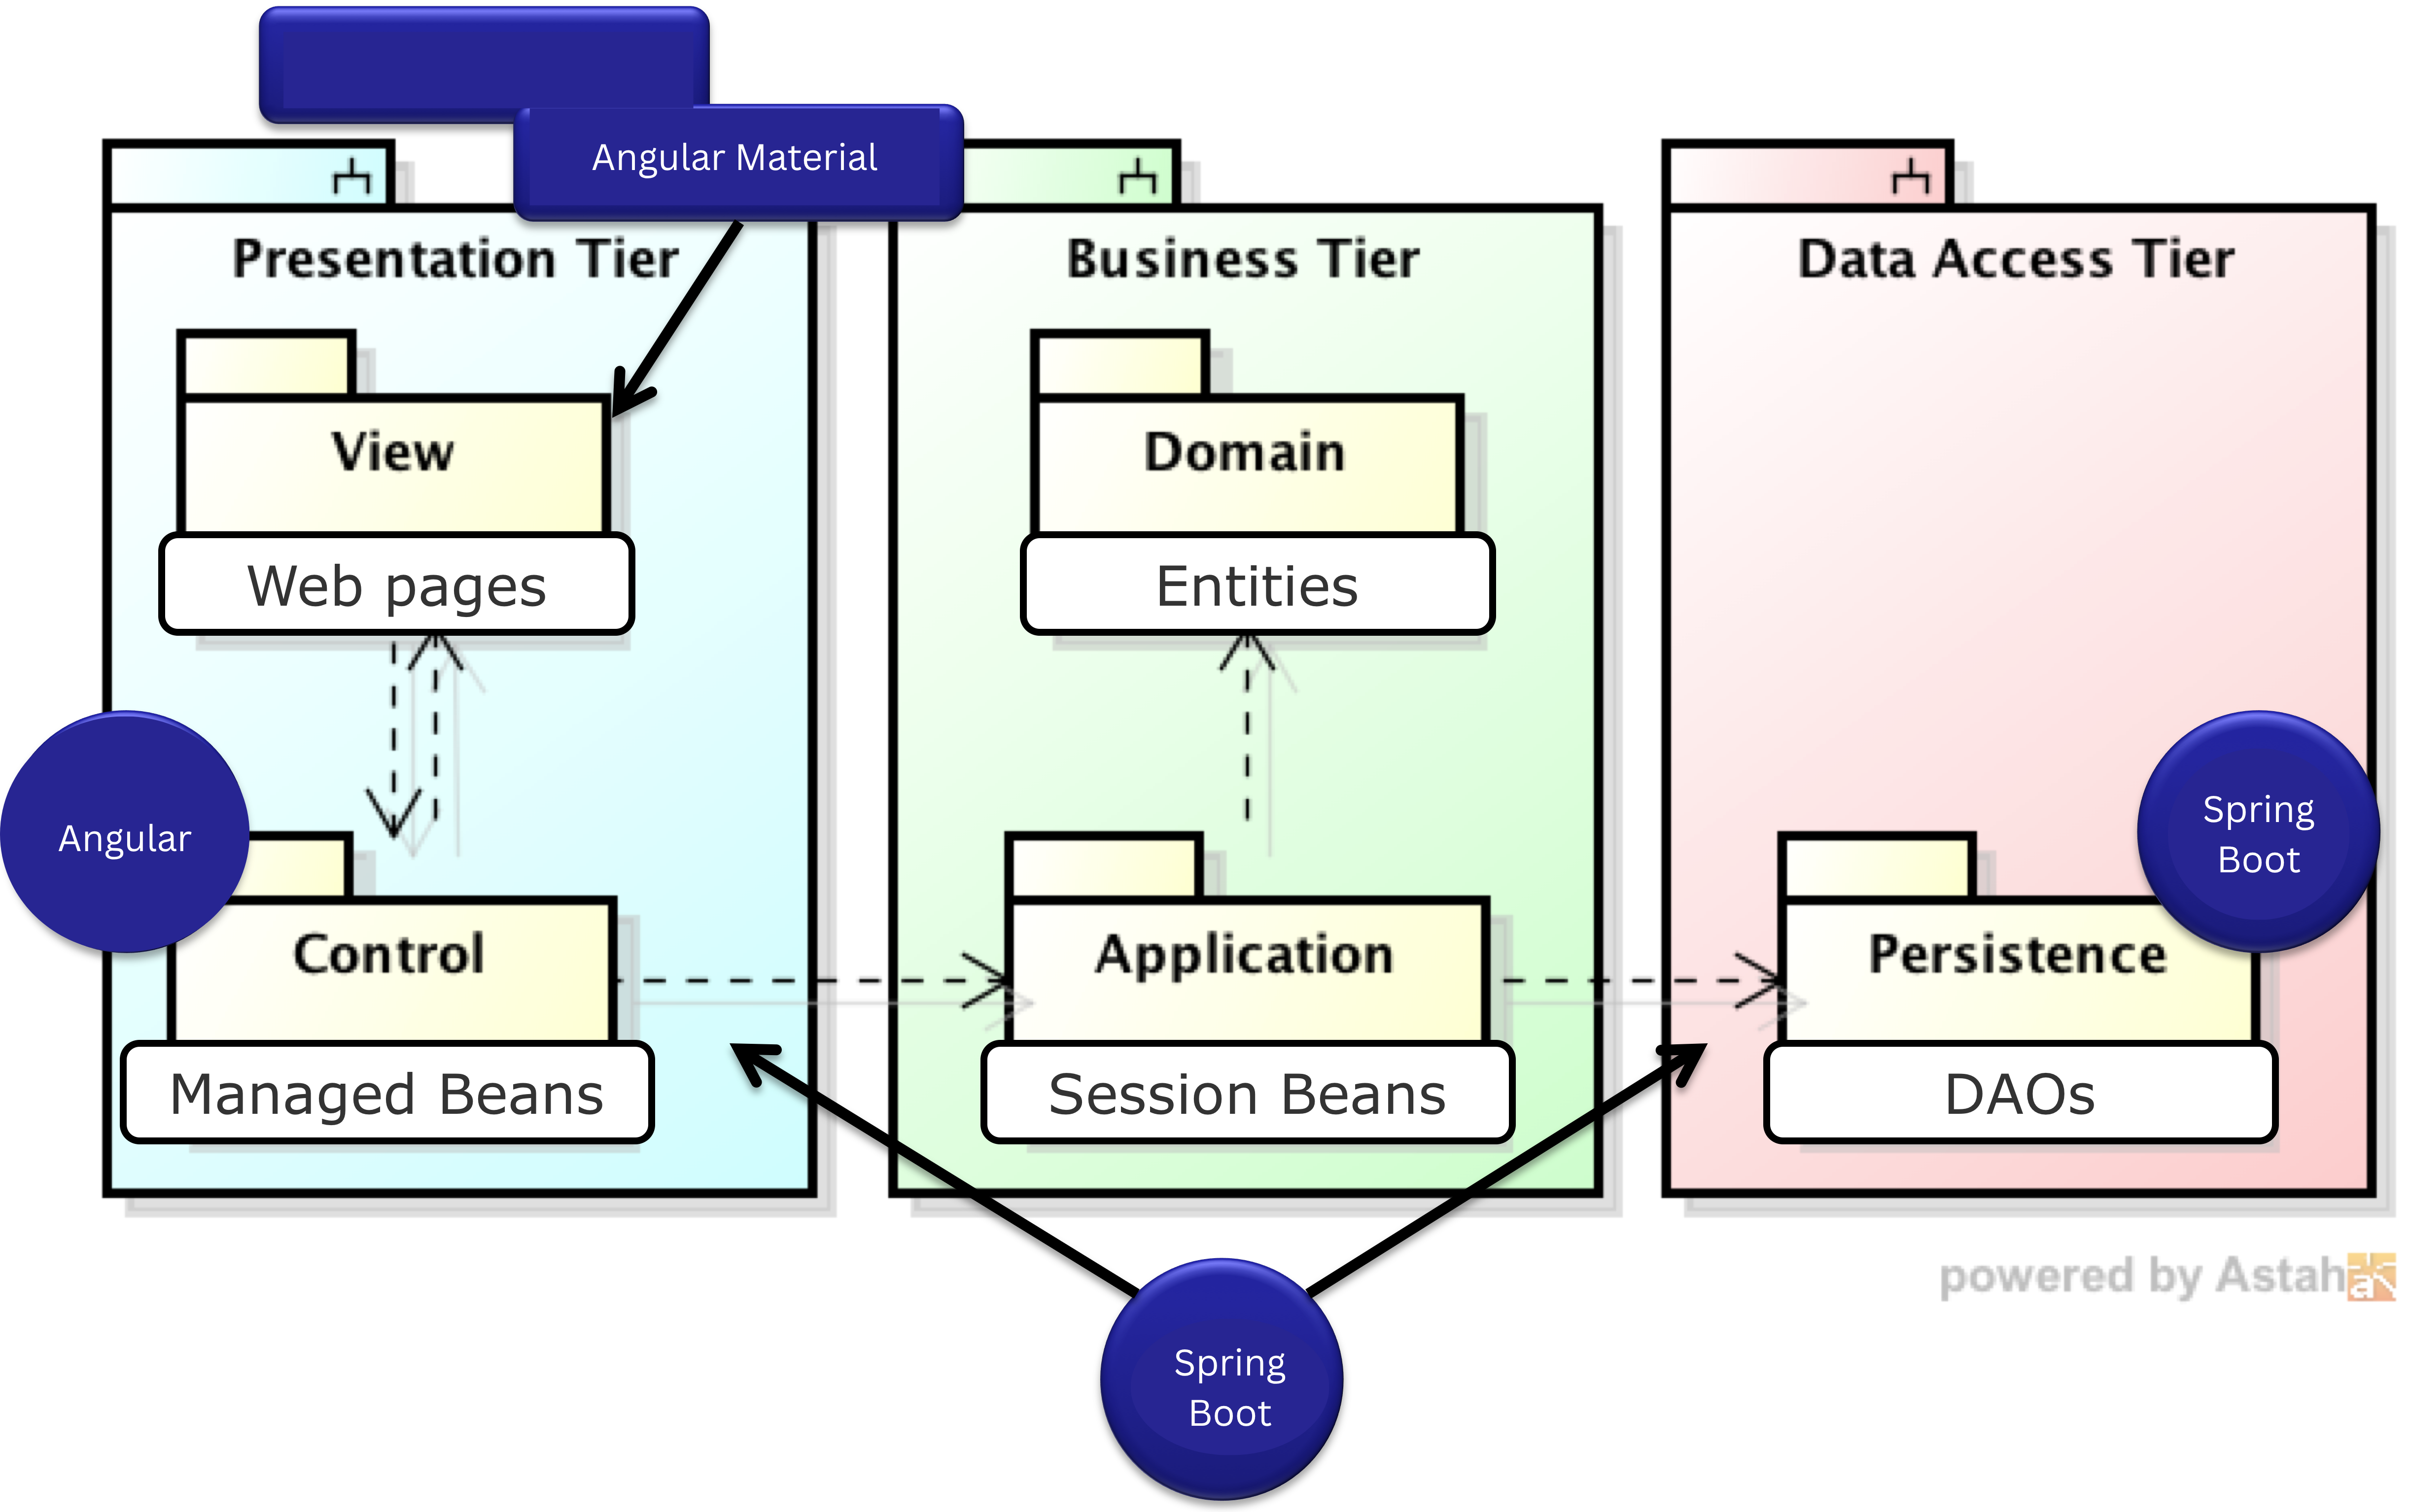
\includegraphics[width=0.8\textwidth]{figuras/arquitetura-frameweb.png}
	\caption{Arquitetura de Software.}
	\label{figura-arquitetura}
\end{figure}

A Figura~\ref{figura-arquitetura-campus} mostra a arquitetura de microsserviços orientada a eventos do back-end \emph{\imprimirtitulo}. Na figura o lado do front-end é abstraído por "Web" com a indicação do ícone do Angular. As requisições do front-end passam por um \textit{Gateway} utilizando o \textbf{Kong Gateway}, em que este direciona as requisições para os devidos microsserviços, fazendo o \textit{load balancing}, distribuindo a carga de requisições entre as instâncias de cada microsserviço. À direita do \textit{Gateway} estão os microsserviços representados por caixas múltiplas (indicando poder ter mais de uma instância) e com a tecnologia de implementação indicada pelo ícone do Spring Boot ou da linguagem Go. Cada microsserviço tem o seu banco de dados (também com indicação de ícones da tecnologia), para que os contextos e cargas não se misturem, com a exceção do \textit{Notification} em que sua responsabilidade é de enviar \textit{e-mails} através dos serviços \textbf{Amazon SES}. A comunicação entre o \textit{front-end} e \textit{back-end} se dá via \textbf{API RESTful}. O microsserviço \textit{Media} faz o envio das imagens cadastradas no sistema para o serviço em nuvem \textbf{Amazon S3} e armazena seus dados no banco \textbf{DynamoDB}, que também é um serviço da nuvem da \textit{Amazon}. Entre os microsserviços, a comunicação pode ocorrer de forma síncrona por \textit{API RESTful} ou de forma assíncrona pela \textit{Kafka}.

\begin{figure}[h]
	\centering
	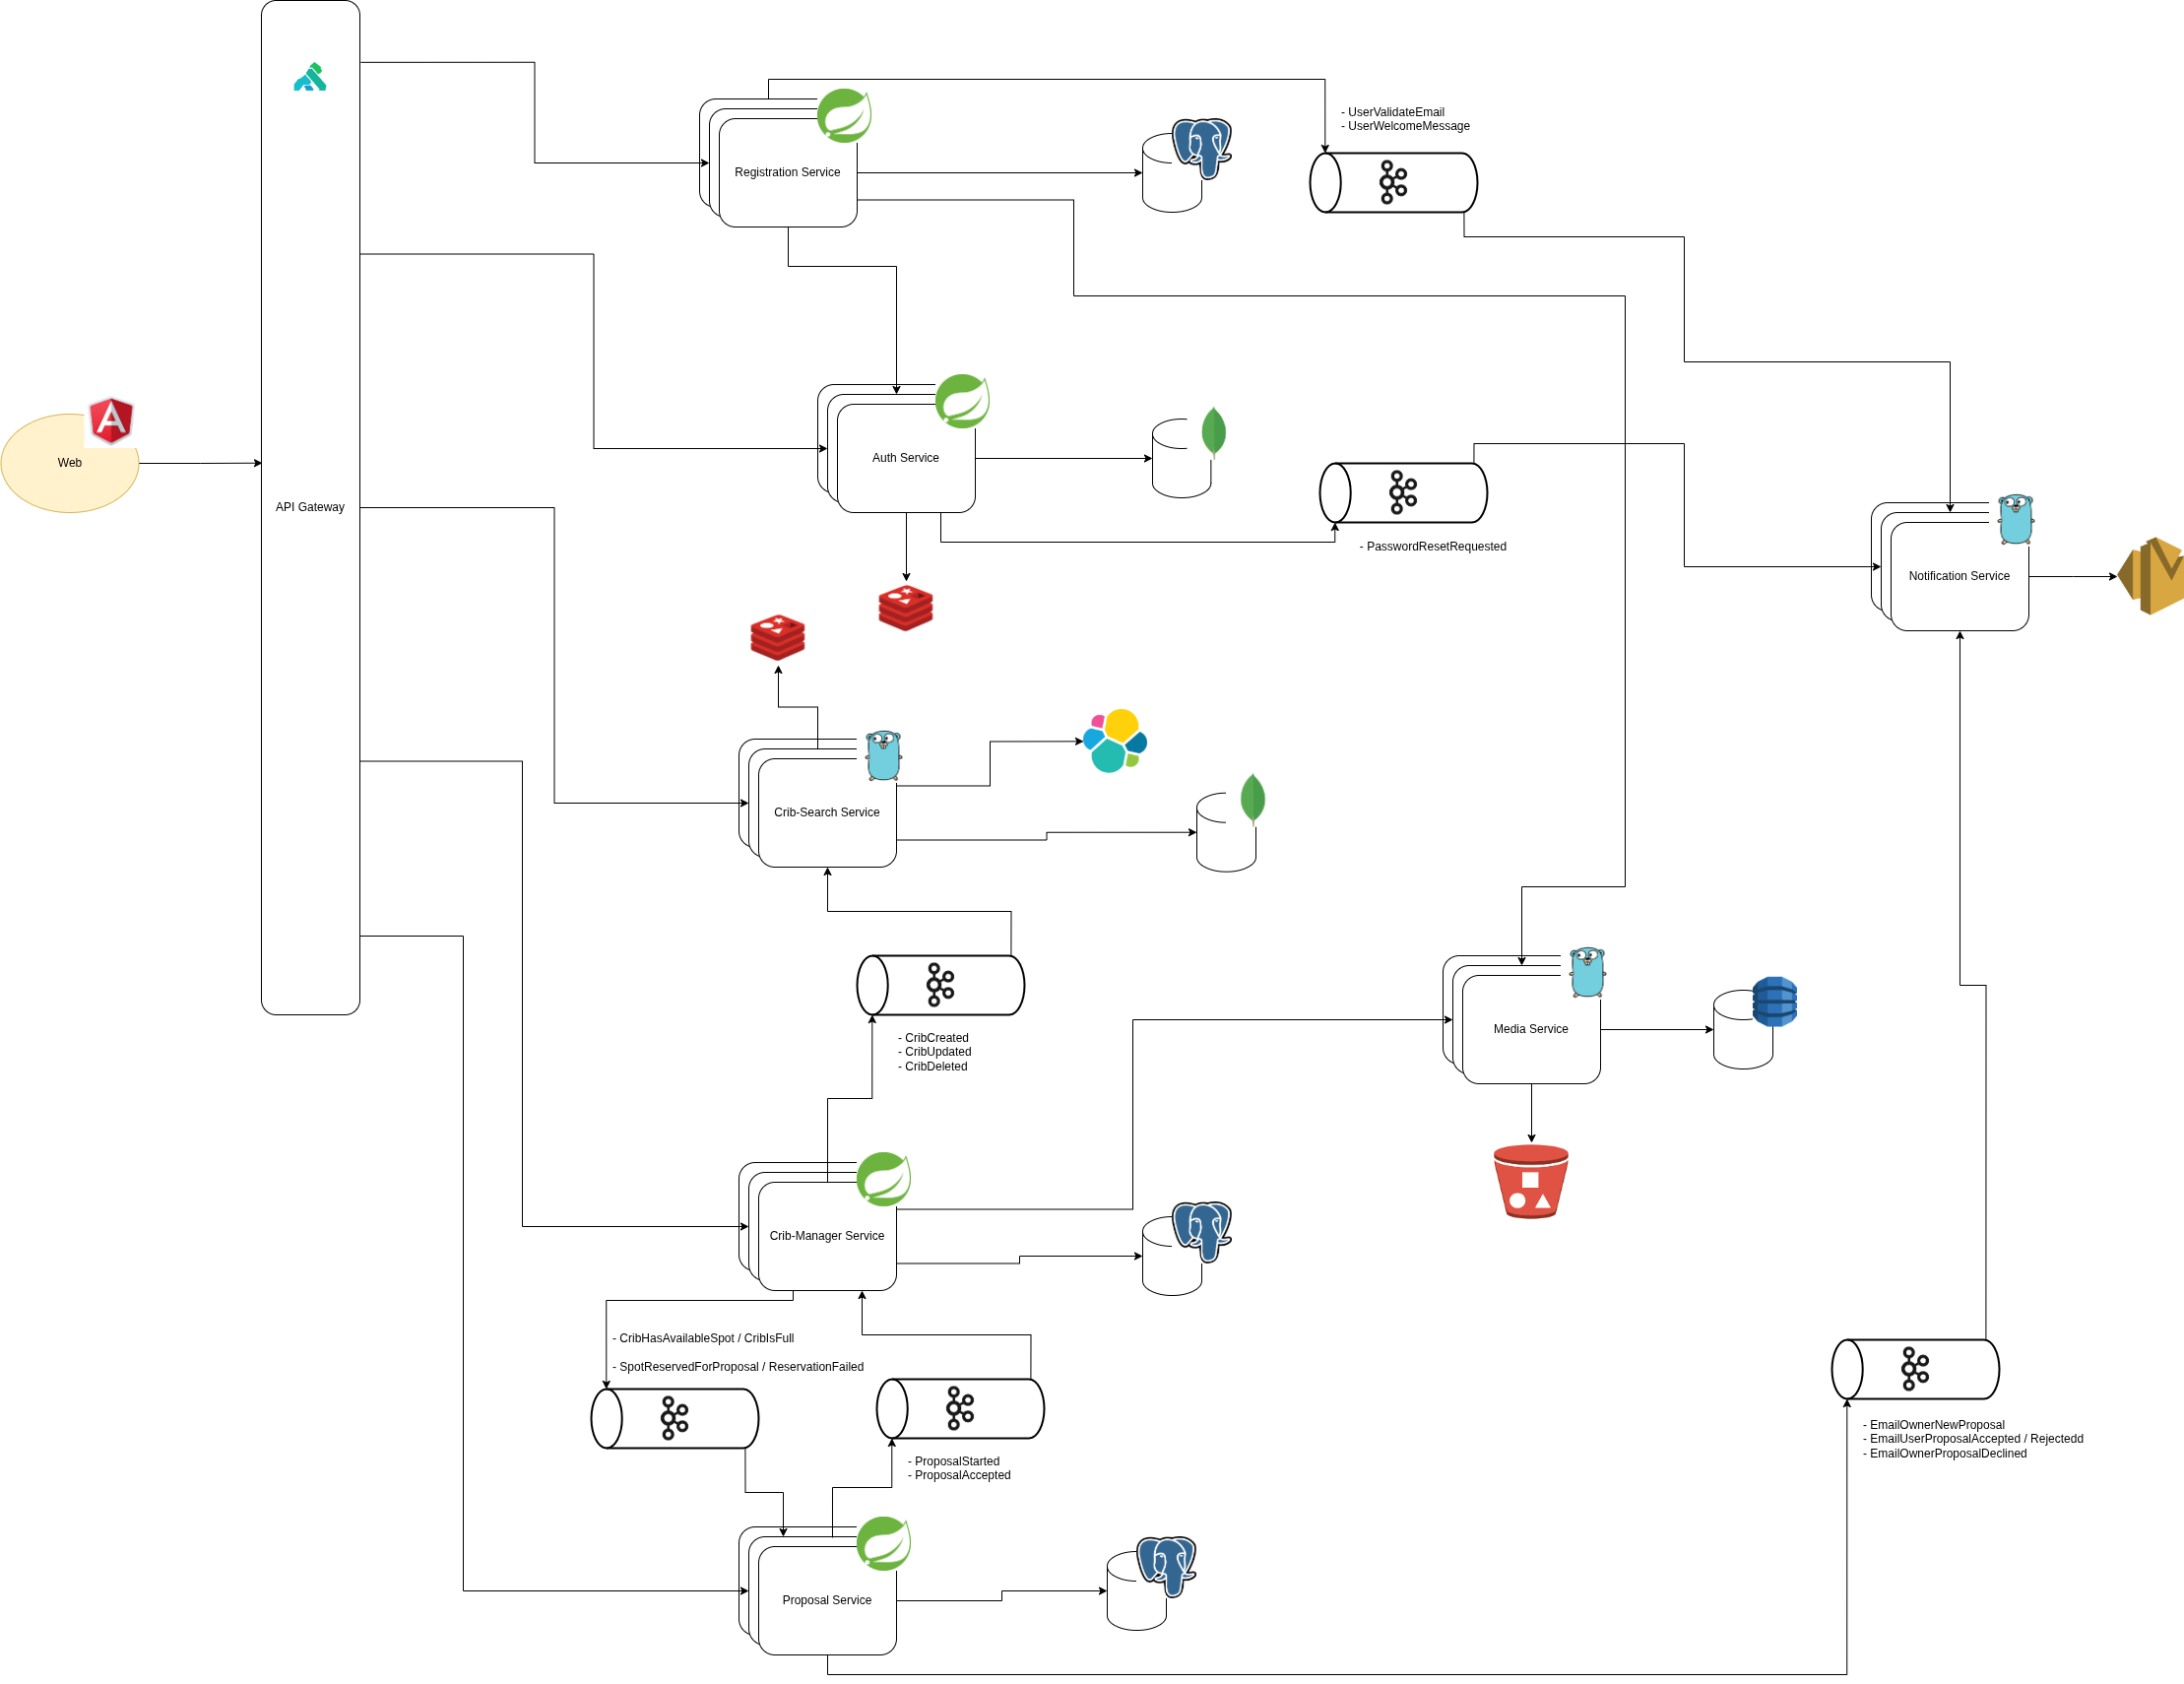
\includegraphics[width=0.8\textwidth]{figuras/campuscrib-diagram-system-design-macro.drawio.png}
	\caption{Arquitetura do Back-End do Sistema}
	\label{figura-arquitetura-campus}
\end{figure}




\vspace*{1.5cm}


\chapter{Modelagem FrameWeb}
\label{sec-frameweb}
\vspace{-1cm}

\emph{\imprimirtitulo} é um sistema Web cuja arquitetura utiliza \textit{frameworks} comuns no desenvolvimento para esta plataforma. Desta forma, o sistema pode ser modelado utilizando a abordagem FrameWeb~\cite{souza-celebratingfalbo20}.


\begin{footnotesize}
	\begin{longtable}{|c|c|}
		\caption{\textit{Frameworks} da arquitetura do sistema separados por categoria.}
		\label{tabela-frameworks}\\\hline
		
		\rowcolor{lightgray}
		\textbf{Categoria de \textit{Framework}} & \textbf{\textit{Framework} Utilizado} \\\hline 
		\endfirsthead
		\hline
		\rowcolor{lightgray}
		\textbf{Categoria de \textit{Framework}} & \textbf{\textit{Framework} Utilizado} \\\hline 
		\endhead

		Controlador Frontal & Angular \\\hline

		Injeção de Dependências & Spring Boot (via Spring IoC Container) e Go (\textit{vanilla}) \\\hline

		Mapeamento Objeto/Relacional & Spring Boot (Spring Data JPA) e Go (pgx) \\\hline

        Mapeamento Objeto/Documento & Spring Boot (Spring Data MongoDB) e Go (mongo-driver) \\\hline

		Segurança & Spring Boot (via Spring Security) \\\hline
	\end{longtable}
\end{footnotesize}

A Tabela~\ref{tabela-frameworks} indica os \textit{frameworks} presentes na arquitetura do sistema que se encaixam em cada uma das categorias de \textit{frameworks} que FrameWeb dá suporte. Em seguida, os modelos FrameWeb são apresentados para cada camada da arquitetura. Para isso, foram selecionadas algumas funcionalidades para serem representadas nos modelos, as quais são:
\begin{itemize}
    \item a funcionalidade de cadastro e autenticação;
    \item a funcionalidade de buscas das repúblicas, incluindo possibilidade de filtros diversos;
    \item a funcionalidade de gerência das repúblicas dos locadores.
\end{itemize}

\section{Camada de Negócio}
\label{sec-frameweb-negocio}

A camada de negócio é responsável pelas regras de negócio do sistema e possui os pacotes \textbf{Application} e \textbf{Domain}, que são representados pelos modelos de \textbf{Entidade} e de \textbf{Aplicação}.

\subsection{Modelo de Entidades}

O modelo de entidade apresenta os objetos de domínio e suas relações \cite{phdthesis}. Especificamente para o sistema \emph{\imprimirtitulo}, as classes \textbf{Crib}, \textbf{Review}, \textbf{Location}, \textbf{Image} e \textbf{User}, que pode ser \textbf{Tenant} ou \textbf{Landlord}, integram esse modelo, como pode ser visto na Figura~\ref{figura-arquitetura-entidades}. 

Um \textbf{Crib} é o objeto que representa uma república dentro do sistema. Ele contém um \textbf{Location}, que é a entidade responsável por armazenar os dados relacionados às coordenadas. Um \textbf{Crib} pode conter vários \textbf{Reviews}, que são as entidades responsáveis por armazenar os comentários públicos que os moradores, chamados de \textbf{Tenant} no sistema, deixam juntamente com seu \emph{rating}, um valor numérico equivalente a estrelas, como em plataformas como o \textit{Airbnb}~\footnote{https://www.airbnb.com}. O usuário do tipo \textbf{Landlord}, que é o locador dentro do sistema, ao cadastrar um \textbf{Crib}, pode adicionar imagens para que os potenciais moradores tenham uma noção de como é o local por dentro.

\begin{figure}[h]
	\centering
	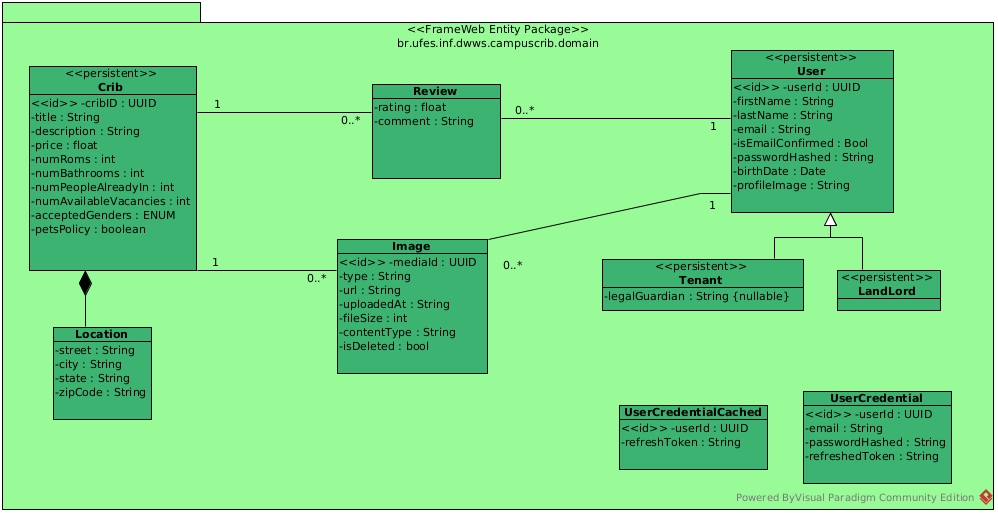
\includegraphics[width=0.8\textwidth]{figuras/modelo-de-entidades.jpg}
	\caption{Modelo de Entidades}
	\label{figura-arquitetura-entidades}
\end{figure}

No modelo de entidade, é possível observar duas entidades que possuem o prefixo \textbf{User}, mas que não apresentam o comportamento de um usuário convencional. Essas entidades existem para representar as informações armazenadas no fluxo de autenticação e autorização. \textbf{UserCredential} representa as credenciais de autenticação de um usuário para a autenticação no padrão JWT~\footnote{https://jwt.io}. O \textbf{UserCredentialCached} é a entidade de cache da credencial de um usuário, em que  o objetivo é de armazenar, em um banco apropriado para cache de dados, um usuário que foi logado recentemente, evitando assim muitas chamadas ao banco de dados que contêm as credenciais.

\subsection{Modelo de Aplicação}

O modelo de aplicação é onde ficam as classes de serviço \cite{phdthesis} e onde ocorre a implementação das funcionalidades e regras de negócio. No modelo, é possível ver as classes controladoras e suas dependências, que são as classes de serviço e as classes de persistência (DAO). 

No sistema \emph{\imprimirtitulo}, adicionamos às interfaces dos serviços o sufixo UseCase para representar a granularidade das operações, que são chamadas em rotas diferentes. Por exemplo, a interface \textbf{CribManagerUseCase}, que representa o serviço \textbf{CribManagerService}. Além de gerenciar a criação e atualização dos Cribs, esse serviço também interage com outros módulos do sistema, como o \textbf{CribSearch}, por meio do método \textbf{sendMessageToCribSearch}. Esse método utiliza um message broker (Kafka) para direcionar as mensagens conforme a necessidade do sistema.


\begin{figure}[h]
\centering
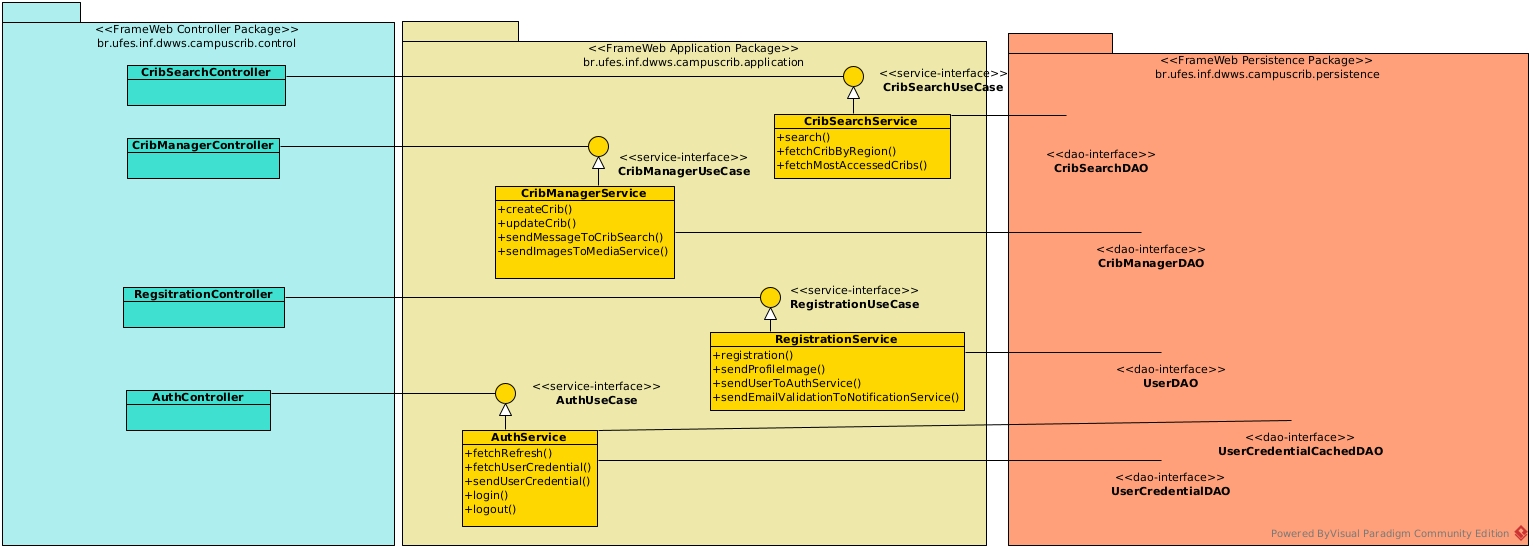
\includegraphics[width=0.8\textwidth]{figuras/modelo-de-aplicacao.jpg}
\caption{Modelo de Aplicação}
\label{figura-arquitetura-aplicacao}
\end{figure}

A figura~\ref{figura-arquitetura-aplicacao} apresenta o modelo de aplicação, em que no centro está (em amarelo) o pacote de aplicação com os serviços e as suas interfaces (casos de uso). A esquerda (em ciano) se tem o pacote control com os controladores em que utilizam os serviços via os casos de uso. A direita (em vermelho) está o pacote de persistência apresentando as interfaces DAO, que são utilizadas pelos serviços.


\section{Camada de Acesso a Dados}
\label{sec-frameweb-dados}

A camada de Acesso a Dados é responsável por gerenciar o armazenamento e a recuperação dos dados do sistema \cite{phdthesis}. Nessa camada, são definidos os repositórios e os objetos que representam as entidades persistidas no banco de dados, garantindo a comunicação entre a aplicação e a base de dados de forma organizada e eficiente.


\subsection{Modelo de Persistência}

O modelo de persistência representa os objetos responsáveis por armazenar os dados gerados pelo sistema. Seguindo o padrão de abstração DAO, esse modelo centraliza todas as interações com o banco de dados, que ocorrem por meio do ORM \cite{phdthesis}.

Os repositórios \textbf{CribSearchDAO}, \textbf{CribManagerDAO} e \textbf{UserCredentialCachedDAO} são interfaces responsáveis pela persistência dos dados relacionados às funcionalidades do sistema \emph{\imprimirtitulo}. O \textbf{CribSearchDAO} é utilizado para a indexação e busca de \emph{Cribs}, enquanto o \textbf{CribManagerDAO} trata da criação, edição e gerenciamento dos \emph{Cribs}, além de contemplar as interações entre usuários e os processos relacionados às propostas. O \textbf{UserCredentialDAO} gerencia as credenciais de acesso dos usuários no sistema e o \textbf{UserCredentialCachedDAO} gerencia as credenciais em cache.

O objeto \textbf{UserDAO} representa a interface de persistência dos dados dos usuários no sistema. Ele contempla todas as operações básicas de criação, atualização, leitura e deleção, bem como funcionalidades específicas associadas aos perfis de \emph{Tenant} e \emph{Landlord} dentro da plataforma.

\begin{figure}[h]
	\centering
	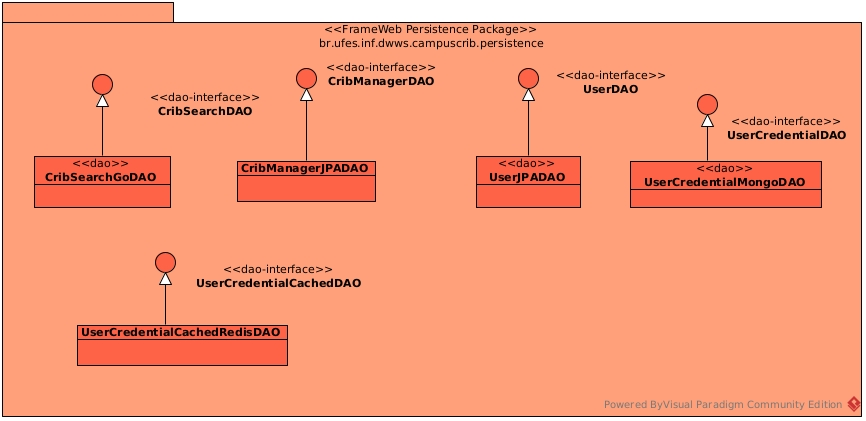
\includegraphics[width=0.8\textwidth]{figuras/modelo-de-persistencia.jpg}
	\caption{Modelo de Persistência}
	\label{figura-arquitetura-persistencia}
\end{figure}

A Figura~\ref{figura-arquitetura-persistencia} apresenta o modelo de persistência do \emph{\imprimirtitulo}, conforme as interfaces supracitadas. Cada uma das interfaces DAO possuem suas implementações, que na figura aparecem relacionadas as interfaces por generalização. Como há diferentes bancos de dados, bem como diferentes linguagens para os microsserviços, então, em \textit{camel case}, a última palavra antes de DAO apresenta qual ORM ou forma de implementar a interface é utilizado. Por exemplo, temos: \textbf{CribSearchGoDAO} implementa \textit{CribSearchDAO} em Go; já \textbf{CribManagerJPADAO} implementa via \textit{JPA} a interface \textit{CribManagerDAO}; para o cache, tem-se \textbf{UserCredentialCachedRedisDAO} implementando a interface \textit{UserCredentialCachedDAO}.


\section{Camada de Apresentação}
\label{sec-frameweb-apresentacao}

A camada de apresentação \cite{phdthesis} é responsável pela parte da aplicação que faz a interface com o usuário, e os modelos de navegação servem para guiar e mapear como será a experiência do usuário com a aplicação.


\subsection{Modelo de navegação Crib Manager}

O modelo de navegação do Crib Manager é o modelo que mostra o processo de gerenciamento dos Cribs dentro do sistema.  
O \textbf{CribManager} é responsável por interagir com os usuários do sistema, criação e atualização do Crib, sendo a parte de gestão das repúblicas de um usuário locador.  

\begin{figure}[h]
	\centering
	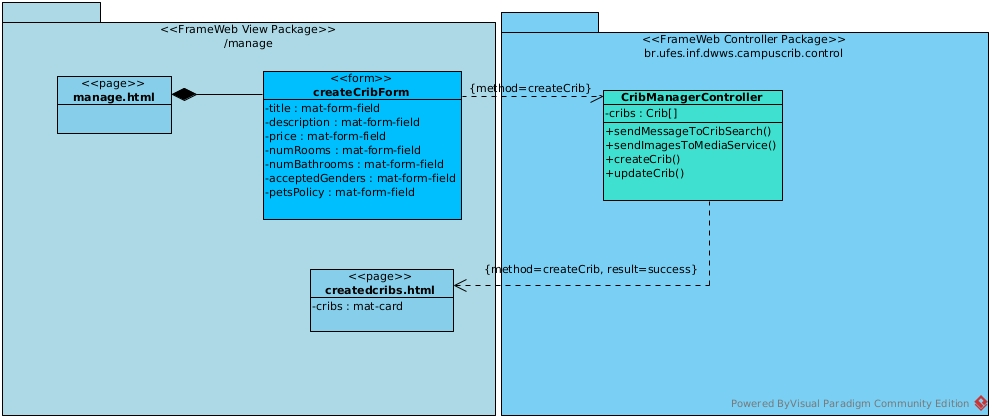
\includegraphics[width=0.8\textwidth]{figuras/modelo-de-navegacao-crib-manager.jpg}
	\caption{Modelo de Navegação Crib Manager}
	\label{figura-arquitetura-nav-crib-manager}
\end{figure}

A figura~\ref{figura-arquitetura-nav-crib-manager} apresenta o modelo de navegação do Crib Manager, em que para o cadastro e edição de uma república tem-se um formulário para enviar os dados da república para o controlador \textbf{CribManagerController}, que retorna as repúblicas do locador, em que são apresentadas por \textit{cards} do Angular Material.

\subsection{Modelo de navegação Crib Search}

O modelo de navegação \textbf{Crib Search}, apresentado na figura~\ref{figura-arquitetura-nav-crib-search}, é o modelo que mostra o processo de busca no sistema. A busca é feita através de um componente \textbf{mat-field} no \textit{front-end}, que gerencia o \textit{input} digitado e o autocomplete para gerar a \textit{query} de busca. A busca pode ser feita por diversos critérios, como por região, que usa a geolocalização informada. Inicialmente, o filtro utilizado é de localização do navegador do usuário atual e, com isso, são trazidos os Cribs que respeitam as condições solicitadas. Os Cribs são mostrados na página através do componente \textbf{mat-card}, que renderiza um Crib e seus dados cadastrados pelo locador (\textbf{Landlord}).

\begin{figure}[h]
	\centering
	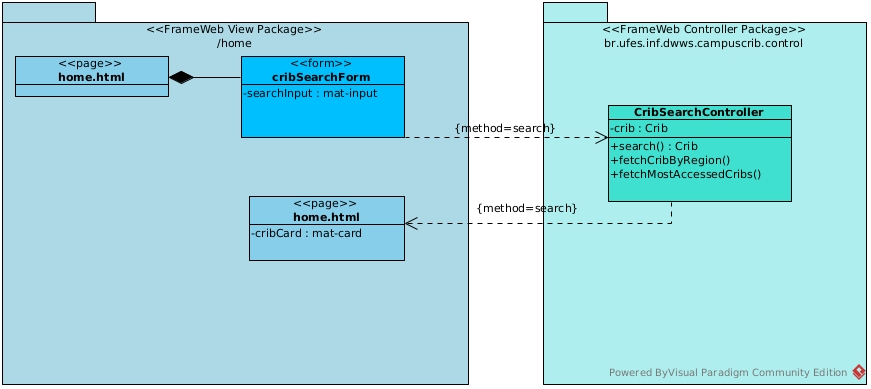
\includegraphics[width=0.8\textwidth]{figuras/modelo-de-navegacao-crib-search.jpg}
	\caption{Modelo de Navegação Crib Search}
	\label{figura-arquitetura-nav-crib-search}
\end{figure}

\subsection{Modelo de navegação Registration/Auth}

O modelo de navegação \textbf{Registration/Auth}, apresentado na figura~\ref{figura-arquitetura-nav-registration-auth}, é um modelo que mostra o processo de criação do usuário e autenticação, que não são dois processos separados, mas complementares dentro do sistema. A criação é feita pelo \textbf{Registration}, que no \textit{front-end} são componentes \textbf{Angular} e um formulário que é enviado para o \textit{back-end}. A camada de controle para nós é a camada de controle do \textit{back-end}. A parte do controlador e serviços do \textit{front-end} são abstraídos no nosso modelo. Essas requisições vão para um \textit{gateway} em que serão direcionadas para o \textbf{Registration Service} (microsserviço responsável pela criação e onde o controlador se encontra).

\begin{figure}[h]
	\centering
	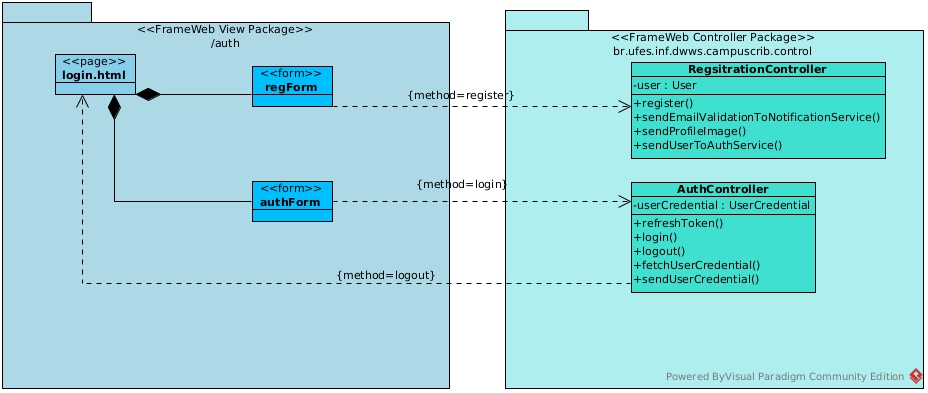
\includegraphics[width=0.8\textwidth]{figuras/modelo-de-navegacao-registration-auth.jpg}
	\caption{Modelo de Navegação Registration/Auth}
	\label{figura-arquitetura-nav-registration-auth}
\end{figure}

Já a parte do login, chamada de \textbf{Auth}, que realiza a autorização e autenticação do usuário, segue o mesmo padrão do \textbf{Registration}, mas também fica responsável pela criação e gerenciamento das credenciais dos usuários do sistema através do padrão JWT.

\endgroup



%%% Páginas finais do documento: bibliografia e anexos. %%%
% Finaliza a parte no bookmark do PDF para que se inicie o bookmark na raiz e adiciona espaço de parte no sumário.
\phantompart

% Marca o início dos elementos pós-textuais.
\postextual

% Referências bibliográficas
\bibliography{bibliografia}

% Índice remissivo.
\phantompart
\printindex

% Fim do documento.
\end{document}
